\chapter{PCA Data Driven Surrogate Signal Extraction Methods for Dynamic PET Full Overview} \label{sec:pca_data_driven_surrogate_signal_extraction_methods_for_dynamic_pet_full_overview_appendix}
    \newpage

    \begin{figure}
        \centering
        
        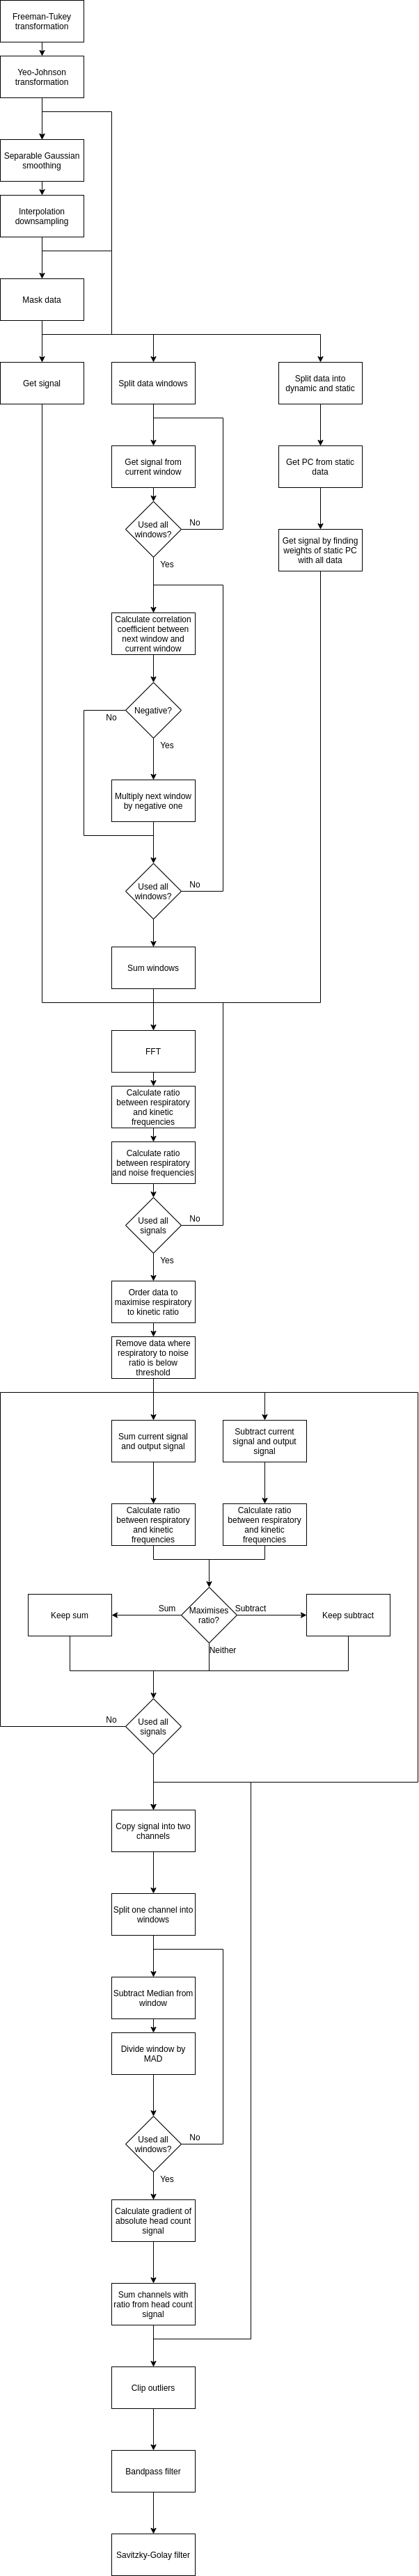
\includegraphics[width=0.2\linewidth]{figures/data_driven_surrogate_signal_extraction_methods_1_full_overview.png}
        
        \captionsetup{singlelinecheck=false, justification=centering}
        \caption{A diagram showing an overview of the possible ways in which the method could be executed.}
        \label{fig:pca_data_driven_surrogate_signal_extraction_methods_for_dynamic_pet_full_overview_appendix}
    \end{figure}
